%%% This is an example file for the Auburn University style options
%%%       aums.sty (Masters Thesis)
%%%       auphd.sty (Ph.D. Dissertation)
%%%       auhonors.sty (Honors Scholar)

%%%To use it, please edit the necessary options, title, author, date, year, keywords, advisor, professor, etc. 

\documentclass[12pt]{report}
\usepackage{aums}       % For Master's papers
\usepackage{ulem}       % underlining on style-page; see \normalem below
\usepackage{url}
\usepackage{tikz}
\usepackage{pgf}
\usepackage{tocloft}     % Use tocloft to introduce single spacing on long chapter name
\setlength\cftparskip{-2pt}
\usepackage[nottoc,notlof,notlot]{tocbibind} 
\usepackage{graphicx}
\usepackage{subcaption}
\renewcommand\cftchapafterpnum{\vskip\baselineskip}  
\renewcommand\cftsecafterpnum{\vskip\baselineskip \normalfont}
\renewcommand\cftsubsecafterpnum{\vskip\baselineskip \normalfont}
\renewcommand\cftsubsubsecafterpnum{\vskip\baselineskip \normalsize}
\renewcommand\cftfigafterpnum{\vskip\baselineskip}
\renewcommand\cfttabafterpnum{\vskip\baselineskip}
\renewcommand{\cftpartleader}{\cftdotfill{\cftdotsep}} % for parts
\renewcommand{\cftchapleader}{\cftdotfill{\cftdotsep}} % for chapters
\usepackage{times}
\usepackage[a4paper,left=1in,right=1in,top=1.15in,bottom=1in]{geometry}
\usepackage{etoolbox}% http://ctan.org/pkg/etoolbox
\usepackage{titlesec}
\titleformat{\chapter}[display] %[display] puts the title chapter on a separate line
  {\singlespace\center}{\chaptertitlename\ \thechapter}{12pt}{\center} % Defines the Chapter title style and size
\titleformat*{\section} {\normalfont\fontsize{12}{12}}  % Added this line to describe section title,numbering and font styles
\titleformat*{\subsection} {\normalfont\fontsize{12}{12}}% Added this line to describe subsection title,numbering and font styles
\titleformat*{\subsubsection} {\normalfont\fontsize{12}{12}}% Added this line to describe subbsection title,numbering and font styles

%%%%%Format rules: Normal margins are 1 in. If you need to print with 1.5in margins, uncomment the line below
%\oddsidemargin0.5in \textwidth6in

%% If you do not need a List of Abbreviations, then comment out the lines below and the \printnomenclature line.
%%for List of Abbreviations information:  (see http://www.mackichan.com/TECHTALK/509.htm  )
\usepackage[intoc]{nomencl}
\renewcommand{\nomname}{List of Abbreviations}   	       
\makenomenclature 
%% don't forget to run:   makeindex ausample.nlo -s nomencl.ist -o ausample.nls
%% Also, if 




% May want theorems numbered by chapter
\newtheorem{theorem}{  \normalfont Theorem} [chapter]

% Put the title, author, and date in. 
\title{A Software Signal Simulation of Low Earth Orbit Satellites for Investigative Analysis}
\author{Samuel McDougal} 
\date{Sometime Spring 2023} %date of graduation
\copyrightyear{2023} %copyright year

\keywords{LEO Satellites, USRP, Navigation, Signals of Opportunity}

% Put the Thesis Adviser here. 
\adviser{Scott Martin}


% Put the committee here (including the adviser), one \professor for each. 
% The advisor must be first, and the dean of the graduate school must be last.
\professor{Scott Martin}

\professor{David Bevly}

\professor{Brendon Allen}

\begin{document}

\begin{romanpages}      % roman-numbered pages 

\TitlePage 

\begin{abstract} 
Place the text of the abstract here. Headings come automatically.
\end{abstract}

\begin{acknowledgments}
acknowledgments
\end{acknowledgments}

\begin{singlespace}

\begin{center} 
\renewcommand{\cftchapfont}{}
\renewcommand{\cftchappagefont}{}
\renewcommand{\cfttoctitlefont}{\normalsize}% Remove \bfseries from ToC title
\renewcommand{\cftsecfont }{\normalsize}% Remove \bfseries from section titles in ToC
\renewcommand{\cftsecpagefont}{\normalsize}% Remove \bfseries from section titles' page in ToC
\tableofcontents 
\newpage
\renewcommand{\cftchapfont}{}
\renewcommand{\cftchappagefont}{}
\renewcommand{\cftloftitlefont}{\normalsize}% Remove \bfseries from lof title
\renewcommand{\cftsecfont}{\normalsize}% Remove \bfseries from section titles in lof
\renewcommand{\cftsecpagefont}{\normalsize}% Remove \bfseries from section titles' page in lof
\listoffigures
\newpage
\renewcommand{\cftchapfont}{}
\renewcommand{\cftchappagefont}{}
\renewcommand{\cftlottitlefont}{\normalsize}% Remove \bfseries from lot title
\renewcommand{\cftsecfont}{\normalsize}% Remove \bfseries from section titles in lof
\renewcommand{\cftsecpagefont}{\normalsize}% Remove \bfseries from section titles' page in lof
\listoftables
\end{center}
\end{singlespace}

\printnomenclature[0.5in] %used for the List of Abbreviations
\end{romanpages}        % All done with roman-numbered pages


\normalem       % Make italics the default for \em

 \chapter { Introduction}  % Use \\ for long titles  

\section { \normalfont Motivation}

Low Earth orbit (LEO) satellites for navigation have gained interest as an alternitive source of position, navigation and timing (PNT) to GNSS due to GNSS being susceptible to interferences such as jamming, spoofing, and multipath. Many current LEO satellites are not designed for navigation, however their signals have been exploited for opportunistic navigation. Many of these constellations have data messages that are unknown to the user which makes receiver design difficult. While there are a few high fidelity LEO simulators on the market, they can be expensive. These tools allow for testing of signal types before satellites are launched and signals can be replicated with prior knowledge of the signal. The development of a signal simulation tool that allows for testing of different signal types, satellite constellations, and receiver patterns is a necessaary tool for developing software and hardware receivers for LEO satellites.  

\section { Prior Work }

There are recent studies in positioning techniques with the growing interest in finding navigation possibilities with LEO satellites. Currently, global navigation satellite systems (GNSSs) are an integral part of modern society. Whether it is directions to the grocery store, land surveying, or autonomous vehicles, the knowledge of where something is and where it is supposed to go is important. Current GNSSs, such as Global Positioning System (GPS), use radio frequencies (RF) to determine position and velocity solutions. Methods for calculating positions and velocities from GPS satellites can be found in \cite{misraGlobalPositioningSystem2012}. 

The flexibility of a simulation tool is crucial. It saves time, money, and resources when testing different scenarios. One of the biggest advantages to this simulation tool is the ability to interchange different pieces quickly and efficiently. Whether it is the constellation type, data message, or signal structure, changes can be made easily to accommodate varying test plans. Current navigation simulation tools are mainly focused on GNSSs such as \cite{dongIFGPSSignal2003} and \cite{corbellDesignValidationAccurate2000}. One source, \cite{powellMultipleAntennaSoftwareGPS} designs a signal simulation tool for ``Rapid Testing of Interference Mitigation Techniques" for GPS. In his thesis, Powell outlines structures for creating a low cost signal simulation tool that can be used to test different scenarios. He begins by generating a file of simulation settings. This is followed by a scenario simulation where satellites are propagated, measurements are generated, and the navigation message populated. Next the signal is generated for the satellites in view and the data is stored in a bin file. GNSS signal simulators can also be used to test software defined receivers (SDRs). Powell validates his simulation by comparing the generated signal performance to the performance of a hardware gps receiver and examining the position, velocity, carrier to noise ratio, and Doppler frequencies. Powell found that the simulator described in his thesis was capable of producing realistic single and multi antenna signals. 


One of the main areas of research for LEO satellites is using the Doppler frequency measurements from the LEO satellites in order to gain a navigation solution \cite{hsuAssessmentUsingDoppler2014} \cite{psiakiNavigationUsingCarrier2021}. Doppler positioning has been used in GNSS \cite{bahramiGNSSDopplerPositioning}, and was even the precursor to GPS \cite{TransitSatelliteSpacebased}. The Transit satellite system was initially used for US naval ships to gain a rough position. In \cite{thompsonSingleDifferencedDoppler2021}, Thompson uses a double differenced Doppler technique to position a moving rover with LEO satellites using angle of arrival (AOA) estimates to remove the need of satellite state knowledge. The Argos satellite system uses Doppler measurements for animal tracking \cite{lopezImprovingArgosDoppler2014}
  

Another area of research with LEO satellites is to use their measurements and colaberate with IMUs for opportunistic navigation\cite{khalifeReceiverDesignDoppler2019} and \cite{tanNewMethodPositioning2019}. In \cite{moralesInertialNavigationSystem2018}, the Orbcomm constellation is used to to aid an inertial navigation system (INS) in a tightly-coupled fashion. Here they used the LEO satellite Doppler measurements and TLE files to estimate the position of a moving UAV without GNSS signals. For the experiment, the UAV was without GPS and had 2 Orbcomm satellites. They claim that this navigation framework lowered the UAV final position error by 72 percent when compared to solely using the IMU.

One possibility is to deploy a new constellation in LEO specifically for navigation  \cite{reidSatelliteNavigationAge2020}.


A LEO satellite signal simulator can be useful for testing different signal types, constellation geometries, and possible errors. The results of a simulation are only as good as the simulator itself. While high end signal simulators exist, they can be expensive and require technical prowess to operate. A low cost version can be valuable and still operate at a high level of fidelity with more ease of use. 

\section { Contributions}
This thesis will describe the process of designing a modular simulation tool for LEO satellites. The versitility of the simulator allows the user to test different scenarios. 
The contributions from this thesis are listed below:
\begin{itemize}
    \item Description of LEO satellite signal simulation tool that generates realistic IQ signals to be used for currrent and emerging constellations
    \item Investigation of USRP playback and record to realistic introduce hardware errors
    \item Examine possible positioning techniques for TDMA signals
    
\end{itemize}

\section{Thesis Outline}
In Chapter 2, the background of satellite orbits, signal types, and modulation types are discussed. In Chapter 3, the simulation tool is described in detail. Chapter 4 dives into the simulation and testing configurations used for this thesis. The results from the testing configurations are discussed in Chapter 5. Conclusions and future work are discussed in Chapter 6 followed by a list of references and an Appendix.


\chapter{Background}

\section{Satellite Orbit Zones}

With regard to space vehicles, there are three main orbital zones. These zones are low Earth orbit (LEO), medium Earth orbit (MEO), and geosynchronous Earth orbit (GEO). These zones are differentiated by the altitude of the orbit above the surface of the Earth. Due to the nature of the orbits, the satellites in these orbital zones have varying mission types. Figure \ref{fig:satorbzone} gives a reference to each of the orbital zones. 

\begin{figure}
    \centering
    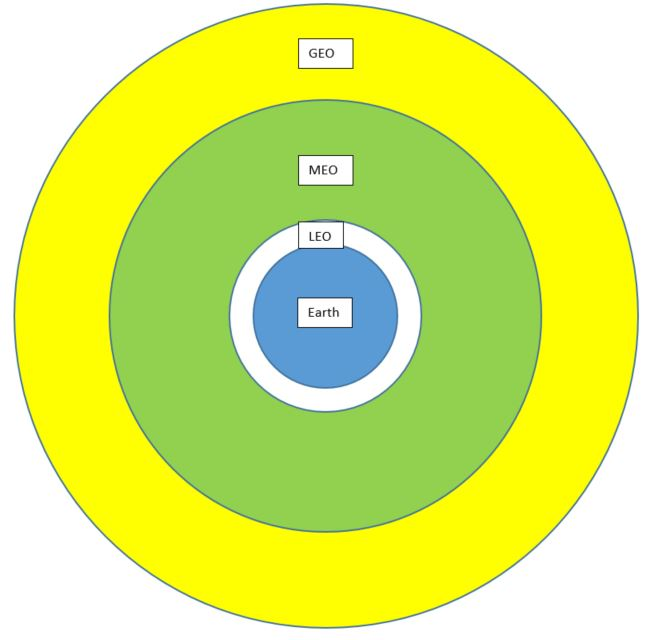
\includegraphics[width=4in]{satellite_orbit_zones.JPG}
    \caption{Visual Representation Orbit Zones}
    \label{fig:satorbzone}

\end{figure}


The furthest of the orbit zones is GEO. These satellites have an orbit altitude of 35,786 kilometers. Geosynchronous orbits are positioned at this precise altitude to allow the satellite orbit period to equal the same time as the rotation of the Earth for one day. The length of the orbit lasts one sidereal day. To an observer on Earth, the satellite would appear to stay in the same place throughout the course of its life. Another form of geosynchronous orbit is the geostationary orbit. Geostationary orbits are geosynchronous orbits specifically located at the Earth's equator and have a near zero inclination angle. GEO satellites are stationed where they are due to their specific mission type. One of the best attributes a GEO satellites has is a large footprint. The large footprint, along with the twenty four hour coverage, means these satellites are great for Earth observation. This also means that fewer satellites are required to be in orbit for full Earth coverage. Many of the current GEO satellites are used for weather, climate surveying, and oceanic observations \cite{usdepartmentofcommerceSatellites}. The Geostationary Operational Environmental Satellites (GOES) are the current Earth observation satellites operated by NASA and NOAA \cite{garnerGOESOverviewHistory2015}. GEO satellites are not conducive for navigation. This is due to the nature of the orbit. Since the orbit is so high, gaining a precise navigation message can be difficult due to loss of signal power and the amount of time it takes for the signal to reach Earth. Another issue with GEO satellites is the cost of launching these satellites. Launching satellites into GEO can cary a much higher price than satellites in LEO or MEO. These points were taken into consideration when GPS was first being thought about. (Maybe include an image of GEO coverage).

MEO is an orbital zone between LEO and GEO. MEO satellites have orbit altitudes between 2,000 kilometers and 35,000 kilometers. The orbit period for most MEO satellites is between 10 hours and 15 hours. Most of the satellites in MEO are navigation satellites. These constellations include GPS (USA), Galileo(European), GLONASS (Russia), and BieDou (China). Each country with GNSSs has designed them specifically for their own use. For example, GLONASS has an orbit altitude of 19,000 kilometers with satellites at specific inclination angles in order for the satellites to spend more time in view over Russia \cite{GLONASSInterfaceControl1998a}. GPS occupies MEO for many reasons, one being the number of satellites needed for global coverage. While more satellites are needed in MEO for global coverage than GEO, fewer are required than in LEO. GPS satellites have an orbit period just under 12 hours. With the orbit altitude and orbit period, 24 satellites are needed for global coverage in order to have at least 4 satellites in view to gain a positioning solution. However, with an orbit period of 12 hours, the observed Doppler frequencies of the satellites are low and can lead to poor velocity estimates. Next, LEO satellites are discussed.

\section{Low Earth Orbit Satellites}
LEO satellites are different than the previously mentioned zones. LEO satellites have orbits from 300 kilometers to 1500 kilometers. With this altitude, the orbit periods for LEO satellites tend to be 60 to 90 minutes, however the ammount of time that a satellite may be in view is lower. This poses issues in terms of global coverage. Satellite constellations with orbit periods on this time scale require far more satellites for full global coverage, and even more satellites for a possible navigation constellation. Reid et al says that it would take nearly 300 LEO satellites in order to provide global coverage \cite{reidSatelliteNavigationAge2020}. 
Current LEO constellations, such as Iridium and Orbcomm, are designed for communications. The Iridium constellation uses global coverage for satellite phones, where the Orbcomm constellation uses ``LEO satellites to provide worldwide geographic coverage for sending and receiving alphanumeric packages," \cite{orabiOpportunisticNavigationDoppler2021}. The data messages on these satellites are unknown as they are proprietary to the companies who sent them into space. This makes it difficult to design receivers and evaluate the navigation performance of these signals. However, a customized navigation message can be put on a similar signal. 

\subsection{Current LEO Constellations}
Current LEO constellations were not designed for navigation, specifically. Most are used for satellite communications, internet, and Earth observations. Some of the major constellations in LEO are Iridium/IridiumNEXT, Orbcomm, and Starlink. The IridiumNEXT \cite{IridiumNEXTReview2019}, which will be refered to as Iridium, is a telecomunications satellite network that comprises of 66 active satellites and 9 in-orbit spares. The 66 active satellites are grouped into 6 orbital planes with 11 satellites in each plane. These satellites are in near polar orbits which means the coverage at the poles is very high, however coverage at the equator is low. The main mission for Iridium is to provide telecomunications with sat-phones. Orbcomm is similar to Iridium as it is a satellite communications constellation, however the physical constellation is different. Orbcomm has 48 satellites with varying inclination angles. The Starlink constellation is a satellite broadband internet provider \cite{Starlink}. This constellation utilizes LEO orbit in an effort reduce latency with internet signals. Instead of using typical terestrial based techniques for internet providing, satellites are used to give coverage in places where internet may not be readily available. However to accomplish this goal, a massive constellation of satellites must be deployed. Currently, there are nearly 3,600 Starlink satellites in LEO with more planned for launch. All of these constellations have one thing in common. The original purpose of the mission was not for navigation. 

\section{Channel Access Methods}

Channel access methods are ways of communicating through mediums between multiple devices. Channel access methods allow users to send information back and forth between terminals. Channel access methods are used to manage telecomunications and wireless traffic. As there are multiple users trying to use or access the same information or services, channel access methods are used to differentiate between the users and the information being passed through the mediums. Three forms of channel access methods that will be examied are time division multiple access (TDMA), code division multiple access (CDMA), and frequency division multiple access (FDMA). 

\subsection{Time Division Multiple Access}

Time division multiple access signals use time to differentiate incoming signals. This results in the signal being burst-like in nature and non-continuous between received signals. The carrier frequency, however, can remain the same accross all users. TDMA signals are typically used by telecomunication satellites such as Iridium. These signals are ideal for communications because as the users are separated in time, the possibility of data interference between users is low. A visual representation of a TDMA signal can be seen in figure \ref{fig:TDMAVisual}.
\begin{figure}[h!]
    \centering
    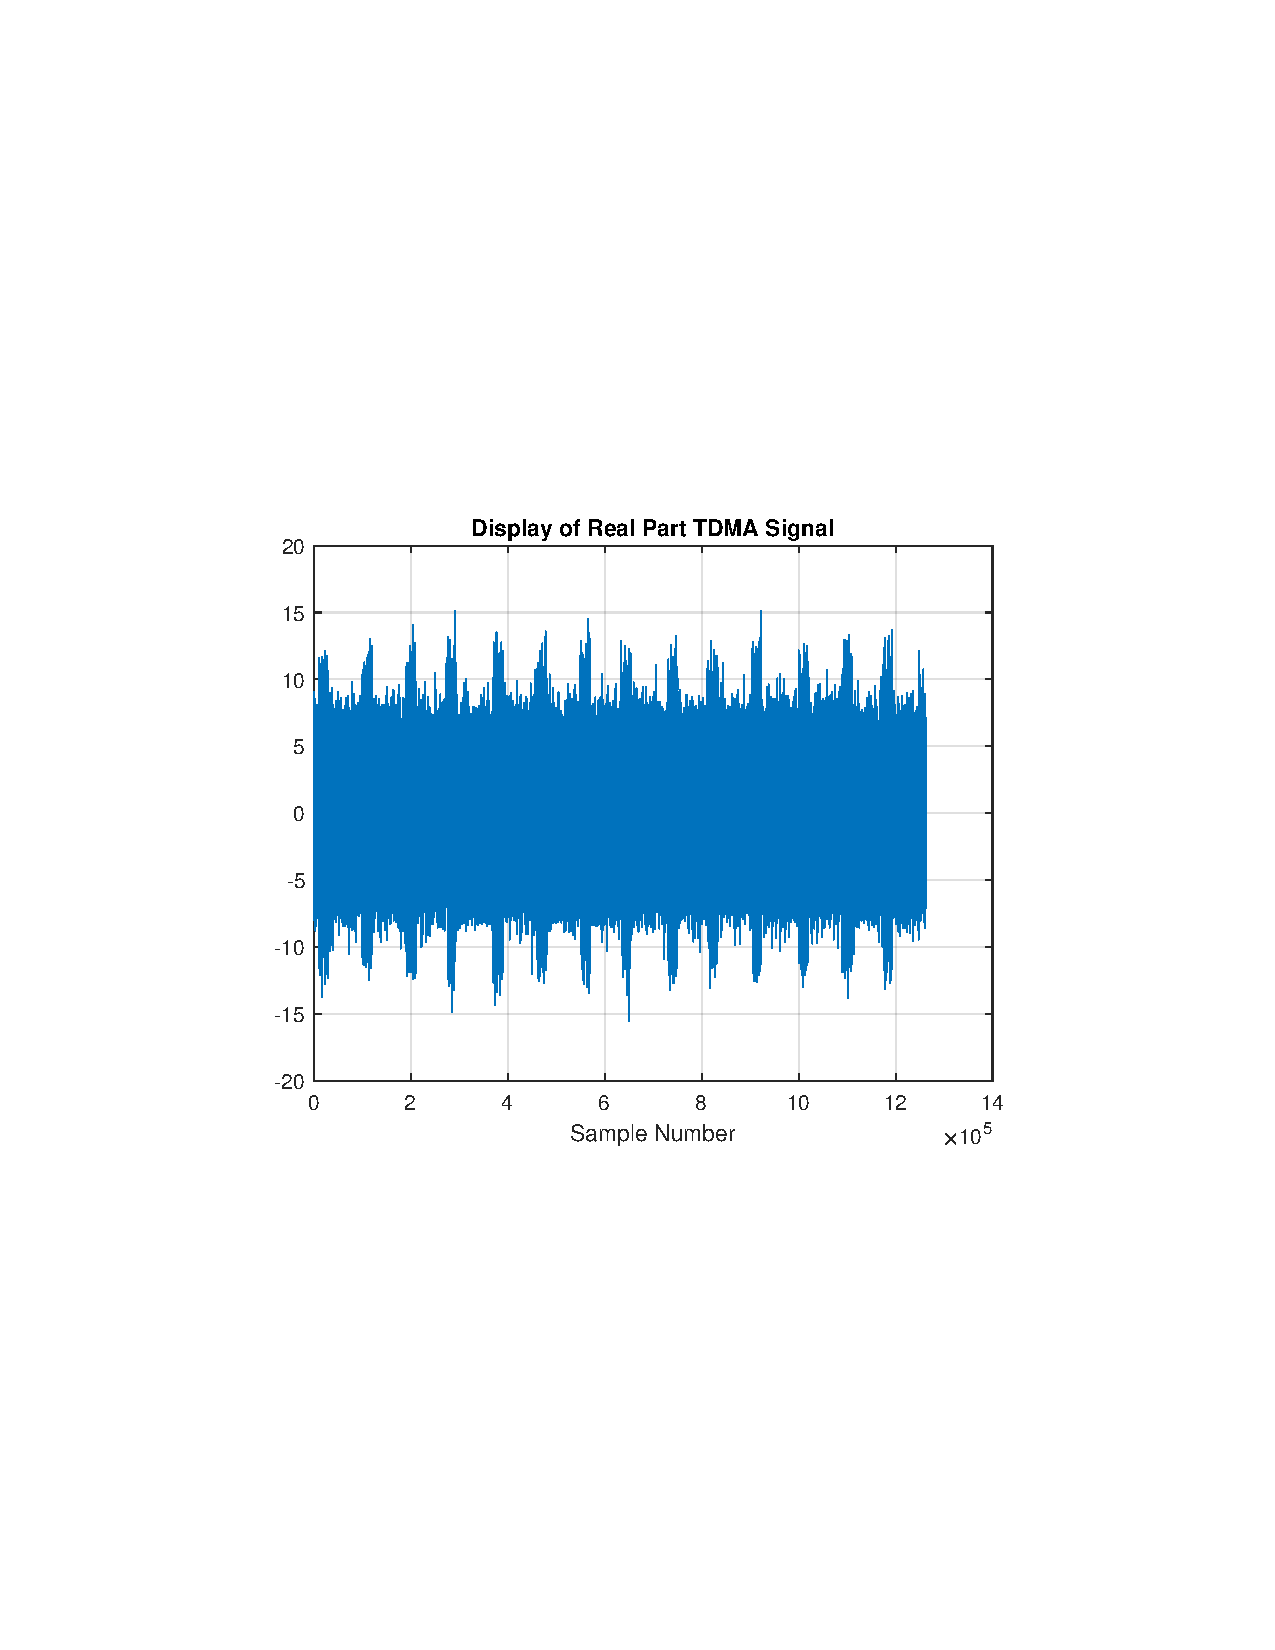
\includegraphics[width=5in]{TDMA_signal}
    \caption{Visual Representation of TDMA Signal}
    \label{fig:TDMAVisual}
\end{figure}
The burst nature of the signal can be seen in this image. The large bulk of the signal is noise, and the parts extending out of the noise are the the bursts. This shows the separation of the signal accross time. 

\subsection{Code Division Multiple Access}

Similar to TDMA, CDMA signals are broadcast at a single carrier frequency. However unlike TDMA, CDMA signals use deterministic binary sequence codes to differentiate signals. In the case of satellites, each satellite is given its own pseudo-random noise (PRN) sequence. These codes are designed specifically to have very low cross correlation in order to eliminate errors and deciphur different satellite's signals in the same frequency band. Cross correlation is a measure of similarity between two or more sequences. They also employ a high level of autocorrelation which is important for signal tracking \cite{goldOptimalBinarySequences1967}. Some notable GNSSs that employ CDMA are GPS and Galileo.

\subsection{Frequency Division Multiple Access}

FDMA signals. What constellations use this signal type, why is it used, how does it opperate. 
Similar to CDMA, FDMA signals are continuous. However, these signals are not transmitted at the same carrier frequency. FDMA signals use different freqency bands to transmit data and information. For example, FM radio uses this technique to differentiate between radio channels such as sports talk radio and the local country music station. Similar to the radio in a car, some satellite constellations use the same idea, except each satellite transmits at a specific frrequency band. For example, GLONASS uses an FDMA for their satellites but also use a PRN code. Unlike GPS, however, they all transmit the same PRN sequence \cite{GLONASSSignalPlan}. 

\section{Modulation}
In the world of satellite navigation and telecomunications, the term modulation refers to the process of incorporating data onto a carrier wave. Three forms of modulation include amplitude shift keying (ASK), frequency shift keying (FSK), and phase shift keying (PSK). ASK is the process of changing the amplitude of the sine wave to represent ones and zeros of binary data, FSK is the process of changing the frequency of the sine wave to represent ones and zeros of binary data, and PSK changes the phase of the signal to incorporate the data. ASK and FSK are shown in figure \ref{fig:ASKsig} and \ref{fig:FSKsig} respectively.

\begin{figure}[h]

    \centering
    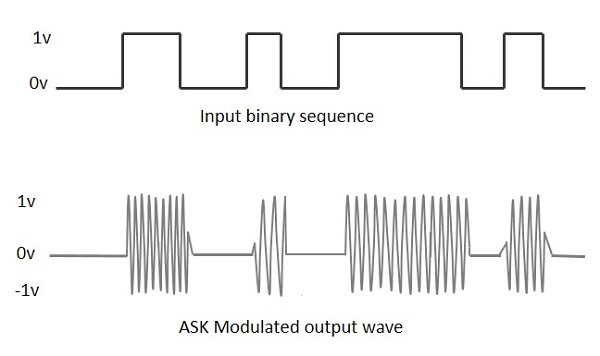
\includegraphics[width=4.0in]{ask_modulated_waveform.jpg}
    \caption{Amplitude Shift Keying Visualization \cite{AmplitudeShiftKeying} }
    \label{fig:ASKsig}

\end{figure}

\begin{figure}[h]

    \centering
    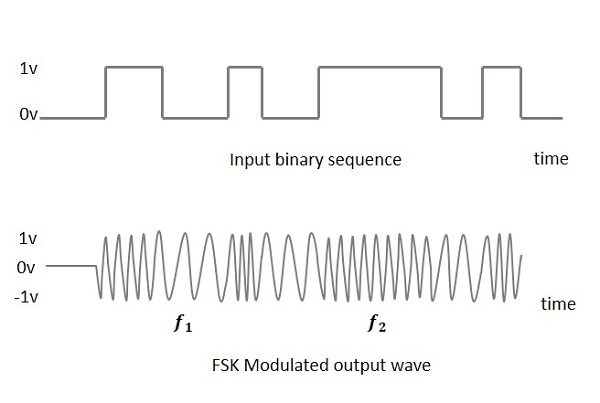
\includegraphics[width=4.0in]{fsk_modulated_output_wave.jpg}
    \caption{Amplitude Shift Keying Visualization \cite{FrequencyShiftKeying} }
    \label{fig:FSKsig}

\end{figure}

Two forms of PSK are binary phase shift keying (BPSK) and quadrature phase shift keying (QPSK) and will be discussed below.

\subsection{Binary Phase Shift Keying}

BPSK is accomplished by shifting the phase of the signal by 180 degrees. By doing so, only one bit can be modulated per symbol. BPSK is used in GPS navigation due to its 
\subsection{Quadrature Phase Shift Keying}

QPSK modulation. QPSK modulation has data on the in-phase and quadrature branches of the signal.

\section{Satellite Based Navigation}
This section will go through some of the basics of satellite navigation. 
\subsection{Trilateration}
\subsection{Ranging Process}
\subsection{Clocks and Accurate Timing}


\chapter {Simulation Tool}
In this section, the function and versitility of the simulator will be described.

\section{Simulator Overview}

The overall structure of the simulation is shown in figure \ref{fig:SimDiagram}.
\begin{figure}[ht]
    \centering
    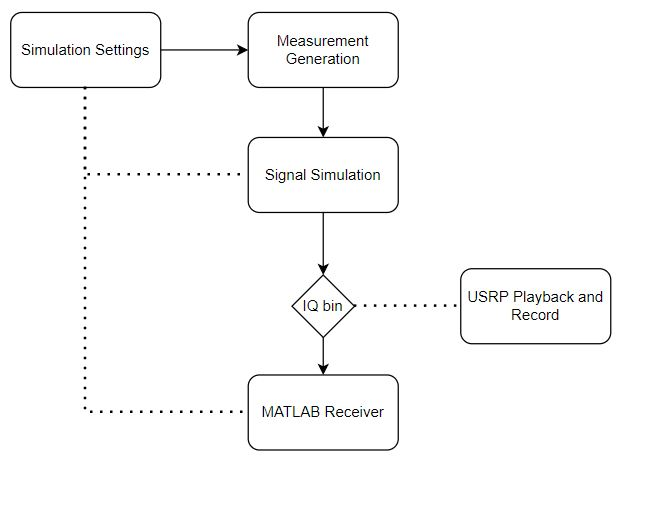
\includegraphics[width=4.0in]{OverallSimulationDiagram}
    \caption{Overall Simulation Diagram}
    \label{fig:SimDiagram}
\end{figure}

The simulation begins with the simulation settings file. This is a configuration file where all of the settings will be declared. This includes, but is not limited to, the satellite trajectories, signal power, and simulation length. The simulation settings file is fed into each block of the simulation tool. First, it goes into the measurement generation block. The measurement generation block is where the satellite positions and velocities are propagated, ranges and range rates are calculated, and transmit and received times are produced. Those terms are pushed into the signal simulation. Inside the signal simulation block the signal is generated and packaged into a bin file. Finally, the bin file is sent to a receiver where it is picked up, processed, and decoded to produce measurements. The following subsections will address each part of the simulation.

\section{Simulation Settings}

The simulation settings is a configuration file where all of the constants and settings used throughout the simulation are declared. All of the settings are stored in a MATLAB structure labeled `settings'. A MATLAB structure is a data storing type where different variables can be tied to one overall variable. The purpose for incorporating all of the settings and variables in one script is to ensure all variables are in one place. This helps the user find a variable quickly and efficiently. It also aids the user by ensuring consistency across all parts of the simulation. 

In part, the simulation settings allow this tool to be modular. The file begins with constants such as the speed of light, rotation rate of the Earth, Earth gravitational constants, and time constants. These will likely stay the same across any and all simulations. Next is the input of user time. This time is in the format of year, month, day, hour, minute, second and determines the start time of the simulation. Following the time starting point is the duration of the simulation in seconds and the measurement simulation sampling frequency in hertz. The next setting is the user position. Currently, the simulation allows for a static receiver with initial position defined in latitude, longitude, and altitude (LLA); however, the addition of a dynamic receiver can be made. Once the LLA position has been defined, the Earth centered Earth fixed (ECEF) position can be calculated. Next is the introduction of measurement error terms. The first set are weather terms for the error caused by the troposphere \cite{misraGlobalPositioningSystem2012}. These inputs are temperature in Celsius and Kelvin, barometric pressure in millibars, and humidity as a percentage. This is followed by clock settings. Here the user declares what type of clock to use and whether the clock error is to be simulated, indicated by an on or off switch. The clock is modeled based on \cite{}. Next is the satellite propagation settings. This simulation uses a simplified general perturbation (SGP) model for calculating satellite positions and velocities. Here the user will input a two line element (TLE) file name along with other information used in parsing the TLE. The propagation settings also includes a mask angle setting. The mask angle input is in degrees and allows the user to reject  satellites under the specified elevation angle. After the satellite propagation settings are the signal settings. Here the user decides the carrier frequency, sampling frequency, code frequency, number of symbols in the data message, and signal type. One specific signal type is time division multiple access (TDMA). A TDMA signal uses time slots in the form of bursts to decipher different signals, whereas frequency division multiple access (FDMA) uses different frequency channels. If the declared signal type is TDMA, then the burst period will need to be calculated. This is followed by the noise and signal power.

The simulation settings file is integral to this simulation tool. All other components of this simulator are dependent on it. These specific dependencies will be explained in detail in the remaining subsections.

\section{Measurement Simulation}
The next block of the simulation tool is the measurement generation. The measurement generation is where the ranges, range rates, and times are calculated. The purpose of this section is to have a set of truth values that will be used later in the simulation. The block diagram for the measurement generation is shown in figure \ref{fig:MeasBlock}.

\begin{figure}[h]
    \centering
    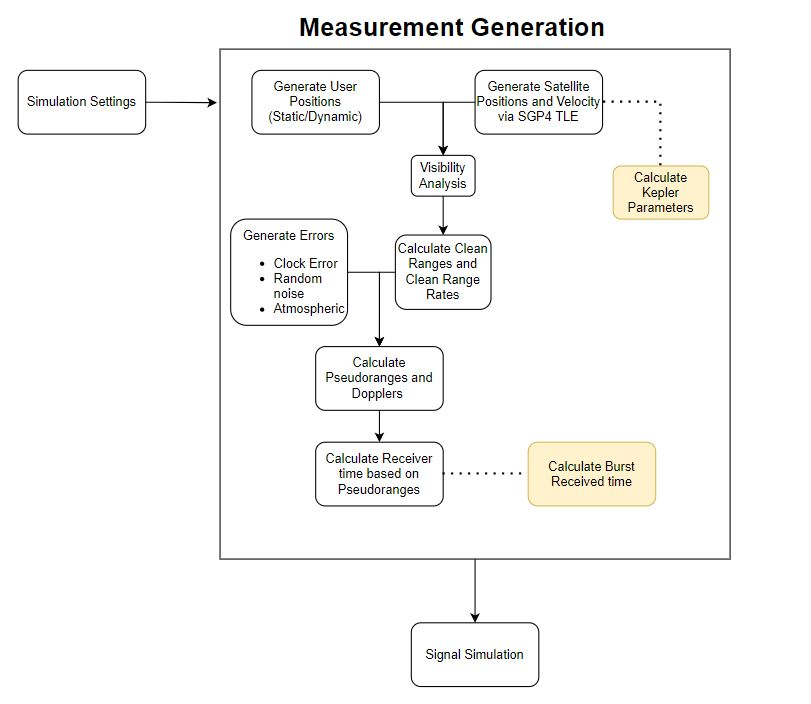
\includegraphics[width=5in]{MeasurementGenBlockDiagram}
    \caption{Measurement Generation Block Diagram}
    \label{fig:MeasBlock}
\end{figure}

The measurement generation begins the same as all  other blocks: inputting the simulation settings file. Again, this allows the user to have all of the same settings, constants, and configurations across all platforms. User positions are generated based on the initial input in the settings file. If a static receiver is declared, then the user position will remain the same and be populated at the set measurement sampling frequency. Along with the population of user positions, satellite positions and velocities are also propagated at this time. For this simulation, a simplified general perturbation (SGP) two line element (TLE) propagator is used to give truth values for satellite positions and velocities. The SGP4 TLE propagator outputs satellite positions and velocities in meters and meters per second, respectively, for the Earth centered inertial (ECI) and ECEF coordinate frames. Figure \ref{fig:bothpropsats} shows the propagated satellite orbits in view for the Iridium and Orbcomm constellations over the duration of the simulation. 

\begin{figure}[ht]
    \centering
    \begin{subfigure}{.4\textwidth}
        \centering
        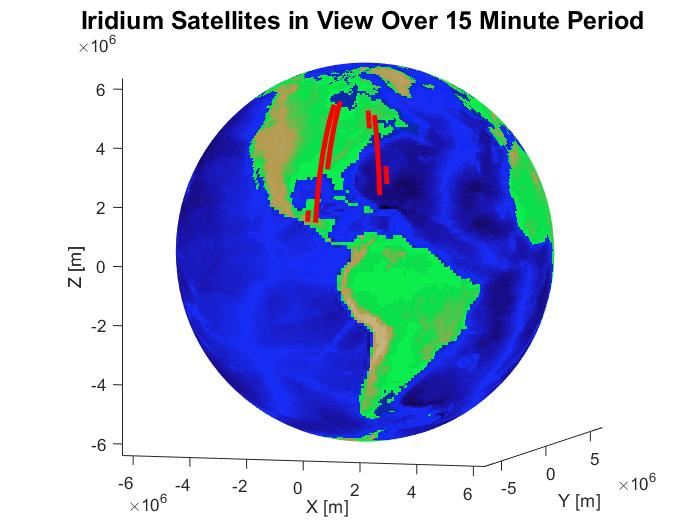
\includegraphics[width=\textwidth]{Iridium_sats_over_auburn.jpg}
        \caption{Propagated Iridium Satellites in View}
        \label{fig:IridSatsOverAub}
    \end{subfigure} %
    \begin{subfigure}{.42\textwidth}
        \centering
        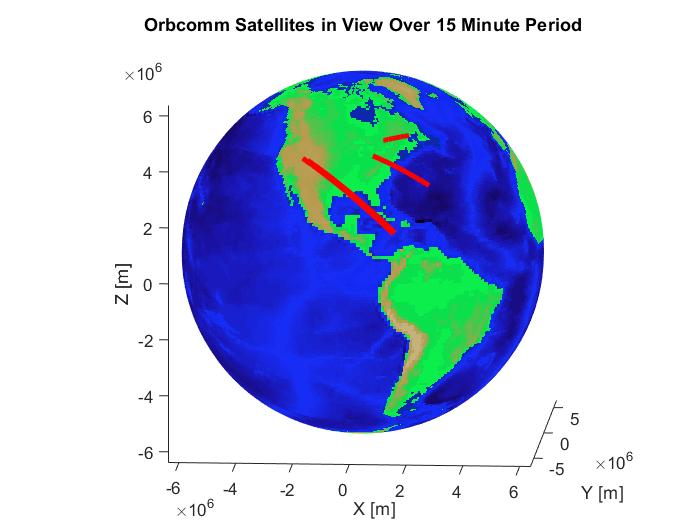
\includegraphics[width=\textwidth]{Orbcomm_sats_over_auburn.jpg}
        \caption{Propagated Orbcomm Satellites in View}
        \label{fig:OrbSatOverAub}
    \end{subfigure}
    \caption{Propagated Satellites from SGP4}
    \label{fig:bothpropsats}
\end{figure}


With both the user position and satellite positions, a visibility analysis can be performed on the satellites. Another important output of the satellite propagation is the elevation angles of the satellites with respect to the user. The visibility analysis takes the elevation angles and finds the satellites that are above the mask angle to eliminate them from the simulation. The output of the visibility analysis is a list of satellites and the times that they are in view. This greatly reduces the computation time for the rest of the simulation because the simulator only has to compute values and signals for the specified satellites that are in view. An option the user has for a data message type is Kepler orbital parameters or classical orbital elements (COE). The calculation of COE uses the ECI satellite positions and velocities calculated previously. These terms are: \textit{h} magnitude of angular momentum; \textit{e} eccentricity; \textit{RAAN} right ascension of the ascending node, \textit{i} inclination angle; \textit{w} argument of perigee; \textit{TA} true anomaly; \textit{a} semi major axis. This process is described in. \cite{curtisOrbitalMechanicsEngineering2008}.

After the visibility analysis, errors will be generated for the satellites that are in view. The first error generated is clock error. Clock bias and drift are generated for the receiver and the satellites. This option can be turned off and the errors will be incorporated as zeros in the simulation. Next the tropospheric delay is calculated from the settings defined previously. Finally, the addition of white Gaussian noise is added for errors not modeled (i.e. Ionosphere delay, multipath, etc). Simultaneously, the true satellite to receiver ranges are calculated along with the range rates. Their equations are show below.
\begin{equation}
    r = \sqrt{(x^{(k)}_{sv} - x_u)^2 + (y^{(k)}_{sv} - y_u)^2 + (z^{(k)}_{sv} - z_u)^2}
    \label{eqn:rangeeqn}
\end{equation}
\begin{equation}
    \dot{r} = (\mathbf{v}^{k} - \mathbf{v}_r) \cdot \mathbf{1}
    \label{eqn:rangerate}
\end{equation}

Having generated ranges, range rates, and errors, the receiver observed pseudorange and Doppler measurements can be calculated. The equations for pseudorange, pseudorange rate, and Doppler are equations \ref{eqn:pseudorange}, \ref{eqn:pseudorangerate}, and \ref{eqn:doppler}, respectively.
\begin{equation}
    \rho^{(k)} = r^{(k)} - b_{sv} + b_r + T +\epsilon
    \label{eqn:pseudorange}
\end{equation}

\begin{equation}
    \dot{\rho} = \dot{r} + \dot{b_r} - \dot{b_{sv}} + \epsilon
    \label{eqn:pseudorangerate}
\end{equation}

\begin{equation}
    f^{(k)}_{Doppler} = \frac{\dot{\rho}}{-\lambda}
    \label{eqn:doppler}
\end{equation}


Where in equation \ref{eqn:pseudorange}, $\rho$ is the observed pseudorange calculated from range \textit{r} to the $k^{th}$ satellite, satellite clock bias $b_{sv}$, receiver clock bias $b_{r}$ in meters, troposphere delay \textit{T},  and additional noise for errors not modeled $\epsilon$. In Equation \ref{eqn:pseudorangerate}, $\dot{r}$ is the calculated range rate, $\dot{b_r}$ is the receiver clock drift, $\dot{b_{sv}}$ is the satellite clock drift, and un-modeled errors $\epsilon$, all with units of meters per second. In equation \ref{eqn:doppler}, $f^{k}_{Doppler}$ is the Doppler frequency of the $k^{th}$ satellite, $\dot{\rho}$ is the pseudorange rate, and $\lambda$ is the wavelength of the carrier. Once the pseudorange and Doppler measurements have been calculated, the observed receive time of the signal can be calculated. It is important to calculate the received time of the signal based on the pseudorange because the signal is generated at the received level. The received time is calculated as 
\begin{equation}
    t_{rx} = t_{tx} + \frac{\rho}{c}
    \label{receivetime}
\end{equation}
where $t_{tx}$ is the transmit time, $\rho$ is the pseudorange calculated in equation \ref{eqn:pseudorange}, and \textit{c} is the speed of light. For a TDMA signal, burst timing needs to be calculated. For example, if the burst timing 70 milliseconds, then a burst will at $t=0s$, $t=0.07s$, $t=0.14s$ and so on. For this instance, the received time of the signal is also calculated on the burst interval using equation \ref{receivetime}.

The final outputs from the measurement generation are pseudoranges, Doppler Measurements, transmit times, received times, satellite positions, and satellite velocities. Classical orbital elements will be another output if the user has declared to use them for the navigation message. Once the measurements are calculated, the signal can be generated.

\section{Signal Simulation}

The signal simulation begins directly after the measurement generation. The current simulation is for a TDMA signal. The beginning of the simulation begins the transmission of a burst. Only one burst occurs within the specified burst period. Figure \ref{fig:SigSimBlock} gives an overview of the signal simulation.

\begin{figure}[h]
    \centering
    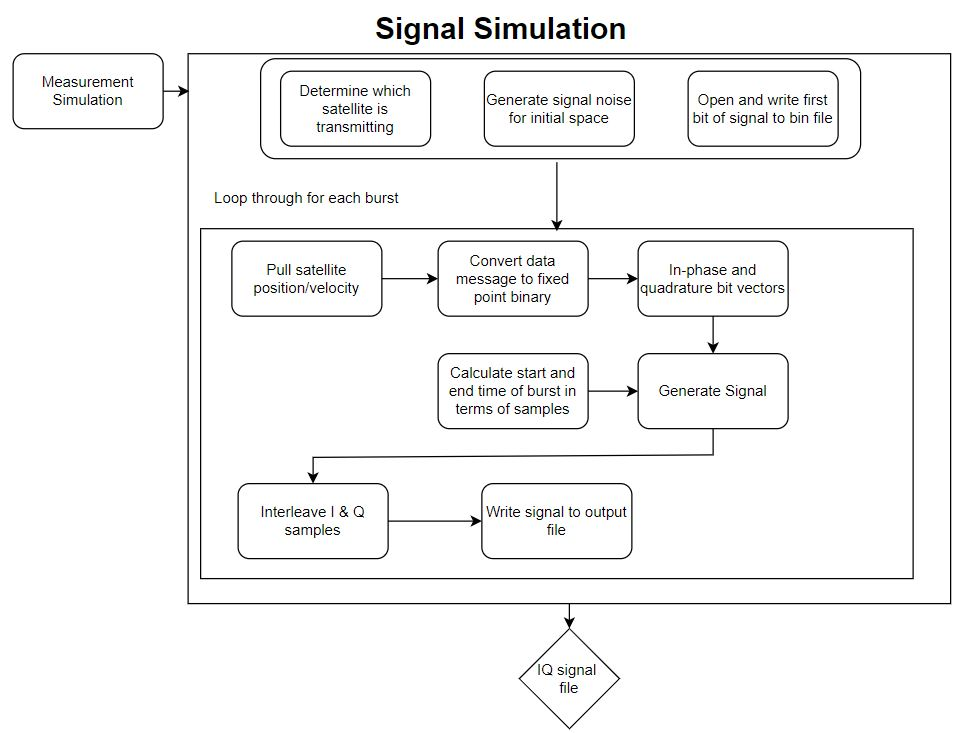
\includegraphics[width=3.5in]{SignalSimBlock}
    \caption{Signal Simulation Block Diagram}
    \label{fig:SigSimBlock}
\end{figure}



The simulation starts by determining what satellite is transmitting and stores it into an array. This process is probabilistic and one satellite in view is chosen at random to transmit. This process is performed for each burst at the start of the signal simulation. Once the burst transmission list has been determined, the first part of the signal is generated. The first part of the output file will be signal noise. The signal noise will be the length of the first transit time in terms of samples. For example, if the first transit time is 0.003009 seconds and the sampling frequency is one megahertz, the first 3009 samples will be noise. Next a bin file is generated and signal noise is written to the file. 

With the calculated received times and designated satellites, we can generate the signal in blocks. We start by gathering the information for the data message. In this case, we gather satellite positions and velocities, satellite number, and transit time. Next, we convert those terms into fixed point binary strings. The data bits are generated in a separate function that is specific to the data message type. The length of each word is predetermined inside the data bit generation function.  The fractional length is determine based on the amount of precision the user desires. The decision to sign the word is also declared.  The outputs of the bit generation function are two row vectors of in-phase and quadrature bits. Non return to zero (NRZ) coding is used to represent the binary ones and zeros. The number of samples in the signal block is determined by examining the begin time of the current burst and the begin time of the next burst. The difference in time is calculated and multiplied it by the signal sampling frequency in order to calculate the number of samples in the block. Next is the generation of the signal shown in figure \ref{fig:SigGenBlock}. 

\begin{figure}[h]
    \centering
    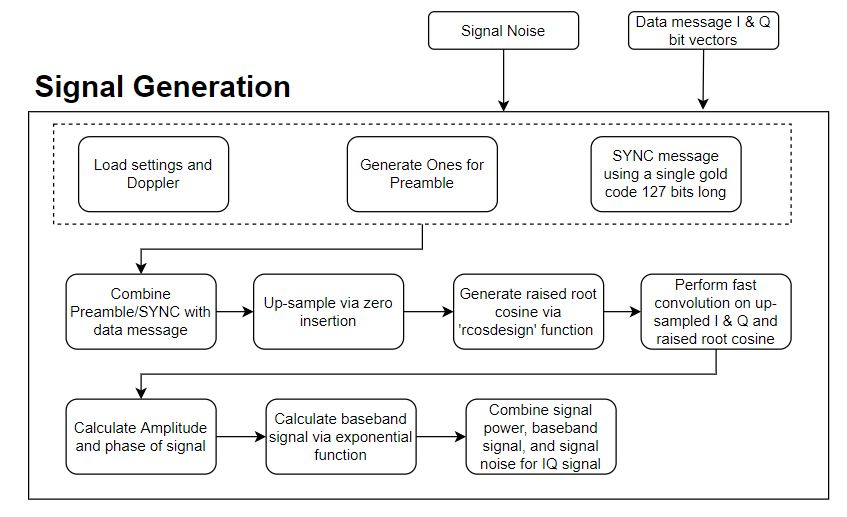
\includegraphics[width=3.5in]{SignalGenBlockDiagram}
    \caption{Signal Generation Block Diagram}
    \label{fig:SigGenBlock}
\end{figure}

A section of signal noise is generated for the amount of samples in the signal block. The signal noise and data message are input to the signal generation block. We start by loading in settings, Doppler frequency, preamble, and sync message. The sync message was chosen to be a 127 bit long gold code with an appended zero due to its autocorrelation abilities \cite{dinanSpreadingCodesDirect1998}.  We then combine the preamble and sync messages on their respective branches along with the in-phase and quadrature bit vectors to produce our full data message. From there we up-sample via zero insertion and filtering with a root-raised-cosine (RRC) pulse shaping filter. The amplitude of the signal is calculated as equation \ref{eqn:amplitude} and the phase is calculated in equation \ref{eqn:phase}

\begin{equation}
    A = \sqrt{Ips^2 + Qps^2}
    \label{eqn:amplitude}
\end{equation}

\begin{equation}
    \theta = tan^{-1} \frac{Qps}{Ips}
    \label{eqn:phase}
\end{equation}
where \textit{Ips} and \textit{Qps} are the pulse shaped in-phase and quadrature branches respectively. The signal is generated through an exponential function in equation \ref{eqn:signal}

\begin{equation}
    A e^{j2\pi (f_{Doppler}t + \theta)}
    \label{eqn:signal}
\end{equation}
where \textit{A} is the amplitude and $\theta$ is the phase. From here the declared signal power is added along side the signal noise. The output of the signal generation function is a full IQ signal with signal noise. The signal is then split into real and imaginary parts, where they are interleaved and written to the bin file. To save computational memory, the signal variables are cleared with each iteration. This process is performed for each block of signal throughout the simulation. At the end of the simulation, if there is a received time outside the bounds of the simulation time, then the simulation will end the file with signal noise.

\section{Receiver}
- Include stuff about burst receiver

- Maximum likilehood burst detection
    - find source for this so I can talk about it in detail.

- Decoding of the bits

- Receiver outputs. Decoded Navigation Message, Doppler Frequency, location of the bit (to get a range), Failed bursts, Successful Bursts, output bits for bit error calculation,

\chapter{Testing Setup and Positioning Techniques}
\section{Doppler Positioning}
\section{Pseudorange Based}
\begin{itemize}
    \item     - Mention things about the configuration:
    \item     - satellite orbits
    \item     - signal type
    \item     - USRP playback and record
    \item     - why important
    \item     - how it works
    \item     - how USRPs work in brief


\end{itemize}


\chapter{Results}
\section{Static Clean Data}
\subsection{Doppler Positioning}
\subsection{Pseudorange Based Positioning}
\section{Static Clean Data Played Through USRP}
\subsection{Doppler Positioning}
\subsection{Pseudorange Based Positioning}
\section{Static Dirty Data}
\subsection{Doppler Positioning}
\subsection{Pseudorange Based Positioning}
\section{Dynamic Clean Data}
\section{Dynamic Clean Data Played Through USRP}
\section{Dynamic Dirty Data}
    - positioning results

    - Doppler Positioning 

    - comparison of constellations 

    - positioning algorithms

    - batch recursive least squares

    - 2d positioning and 3d positioning

    - possible aided doppler positioning techniques

    - How many bursts were detected and accurately decoded

    - Possible testing configurations   
        
        - Full clean data (no clock, no noise, no trop)

        - Full clean data run through USRP 

        - Simulated dirty set with trop error, clock error, sig noise

        - Run this simulation for 2 different satellite constellations

        - See if I have to run it for a dynamic rover 
            - Update:I do.




\chapter{Conclusions and Future Work}
- The simulator works well 

- addition of more signals

- addition of multiple constellation

- addition of more error terms





\bibliographystyle{unsrt}
\bibliography{MyLibrary}






\begin{appendix}
\chapter*{Appendices\addcontentsline{toc}{chapter}{Appendices}}


\begin{singlespace}


\end{singlespace}
\end{appendix}
\end{document}

